\documentclass[conference]{IEEEtran}
\IEEEoverridecommandlockouts
% The preceding line is only needed to identify funding in the first footnote. If that is unneeded, please comment it out.
\usepackage{cite}
\usepackage{amsmath,amssymb,amsfonts}
\usepackage{algorithmic}
\usepackage{graphicx}
\usepackage{textcomp}
\usepackage{xcolor}
\usepackage{float}
\def\BibTeX{{\rm B\kern-.05em{\sc i\kern-.025em b}\kern-.08em
    T\kern-.1667em\lower.7ex\hbox{E}\kern-.125emX}}
\begin{document}

\title{Ineroperability Between Homogenous and Heterogenous Blockchains\\


}

\author{\IEEEauthorblockN{1\textsuperscript{st} Adam Svitek}
\IEEEauthorblockA{\textit{Faculty of Informatics and Information Technology STU)} \\
\textit{Slovak Technic University}\\
Bratislava, Slovakia \\
xsviteka@stuba.sk}
}

\maketitle

\begin{abstract}
This document is a model and instructions for \LaTeX.
This and the IEEEtran.cls file define the components of your paper [title, text, heads, etc.]. *CRITICAL: Do Not Use Symbols, Special Characters, Footnotes, 
or Math in Paper Title or Abstract.
\end{abstract}

\begin{IEEEkeywords}
component, formatting, style, styling, insert
\end{IEEEkeywords}



\section{Introduction}
Blockchain interoperability is one of the essential requirements for modern decentralized systems. What was once mostly a matter of communication between separate blockchain networks has slowly evolved into more complex challenge of execution layers, heterogeneous architectures and different transfer mechanisms. Particularly, Ethereum ecosystem in current state extends beyond the main network (Layer 1) to a fast growing set of Layer 2 solutions that improve scalability and reduce transaction costs. As the number of users and decentralized applications who operates in these environments increases each day, seamless movement of assets between layers and ecosystems becomes an important concern.
\\
\\
Users nowadays may need to transfer assets from Layer 2 to Layer 1 and vice versa or even make transactions to another ecosystem such as Polkadot. Although there are many existing interoperability protocols and bridges already supporting these exchanges and transfers, they each solely focuses on one step of the transfer route.  These mechanisms mostly differs in their interfaces, operations and transaction flow. As a result, multi-step transfers still remains split, technically demanding and prone to more errors.
\\
\\
This paper addresses the described transfer fragmentation problem by proposing a unified transfer flow connecting the Ethereum ecosystem with Polkadot ecosystem. The proposed solution combines two asset transfer mechanisms called Across from Ethereum asset transfers including tranfers within Layer 2 networks and Layer 2 to Layer 1 and vice versa , with Snowbridge as an interoperability bridge between  Ethereum and Polkadot. This way, the solution enables a seamless transfer path from Ethereum L2 environments right to Polkadot through single web based aplication. Rather then forcing user to make more transactions across different web aplications, the proposed system  aims to connect  these interoperability  multi steps into one process



\section{Background}

\subsection{Blockchain}

Blockchain is a type of distributed ledger technology that
enables a network of participants to maintain a shared and
synchronized database without relying on a central authority
\cite{nakamoto2008bitcoin, indjcst-fundamentals}. Transactions are grouped into blocks, which are crypto-
graphically linked to form a chain; hence the name blockchain
\cite{indjcst-fundamentals}.

This structure ensures transparency and immutability,
as altering any stored data would require modifying all
subsequent blocks and gaining consensus from the majority
of the network \cite{nakamoto2008bitcoin}. At the same time, blockchain addresses
fundamental issues of digital systems such as double-
spending, where the same asset could otherwise be used
multiple times without proper verification.

\subsection{Consensus, Proof of Work and Proof of Stake}

Consensus mechanisms are a fundamental building block of
blockchain systems, as they enable agreement on a single valid
state of the network without centralized control. Among the
most widely used mechanisms are Proof of Work (PoW) and
Proof of Stake (PoS), both designed to ensure trust, security,
and consistency in decentralized environments.

Proof of Work was first introduced in 2008 by Satoshi
Nakamoto as part of Bitcoin. Its core idea is that creating
a new block requires solving a computationally intensive
problem. This process involves finding a nonce such that the
resulting cryptographic hash satisfies predefined conditions,
typically a certain number of leading zeros. This method,
commonly referred to as mining, relies on trial and error and
requires significant computational resources.

The security of Proof of Work is based on the high cost of
computation. An attacker would need to control the majority
of the network’s computational power (known as a 51% attack),
which would require substantial investment in hardware
and energy. However, this approach has notable drawbacks,
including high energy consumption, limited scalability, and a
tendency toward centralization through mining pools.

To address these limitations, Proof of Stake was introduced
as an alternative consensus mechanism. Instead of relying on
computational work, PoS is based on economic commitment.
Participants, known as validators, are required to lock a certain
amount of cryptocurrency as stake.

In this model, the probability of being selected to propose
a new block depends on the size of the validator’s stake.
Once selected, the validator proposes a block that is verified
by other participants in the network. Security is ensured
through economic incentives, where dishonest behavior can
lead to penalties such as slashing. Compared to Proof of Work,
this approach significantly reduces energy consumption and
improves scalability, while lowering hardware requirements.
However, it introduces challenges such as potential centraliza-
tion and increased protocol complexity.

\subsection{Blockchain interoperability}

Despite the security and reliability provided by consensus
mechanisms, blockchain systems often operate as isolated
environments, each defined by its own protocol, consensus
rules, and execution model. This lack of standardization
significantly limits their ability to communicate with one
another, leading to interoperability challenges across different
blockchain ecosystems \cite{oajaiml-interop, ceur-interop}.

Blockchain interoperability refers to the ability of inde-
pendent blockchain networks to exchange data and assets
while maintaining security and correctness. As blockchain
ecosystems evolve independently with different architectures
and execution environments, enabling communication between
them has become a key requirement for broader adoption of
decentralized technologies \cite{iet2022, mdpi2022}.

Interoperability solutions aim to bridge these isolated sys-
tems by enabling cross-chain communication. This includes
asset transfers, message passing, and verification of state
across different blockchains. Various approaches have been
proposed, including notary schemes, relays, sidechains, and
hash-locking mechanisms, each introducing trade-offs in terms
of security, trust assumptions, and performance \cite{acm2023}.

From a functional perspective, interoperability enables
cross-chain asset transfers and supports decentralized applica-
tions operating across multiple blockchain networks. However,
achieving such interoperability is non-trivial, as it requires
coordination between heterogeneous systems that may differ
in their trust models, consensus rules, and execution logic
\cite{iet2022, acm2023}.

Despite significant progress in research and development,
many interoperability solutions remain limited to specific net-
work pairs or use cases. As a result, users often need to interact
with multiple systems, increasing operational complexity and
introducing additional risks \cite{mdpi2022, acm2023}.

\subsection{Cross-chain vs Cross-layer}

Cross chain and cross-layer represents two different ap-
proaches to communication within one and across another
blockchain system with each addressing distinct challenges
connected to interoperability and scalability.

Cross chain communication refers to interaction between two or more independent blockchain networks such as Ethereum and Polkadot. Because of their independence they do not share the same consensus mechanism, state, or execution environment.

To partly solve this issue, various solutions were developed such as notary-based systems or lock-and-mint mechanisms. These approaches introduce trade-offs between trust assumptions, security, and complexity.

Cross layer is on the other hand a way of communication across the same network across multiple layers. The network is mostly structured into base layer referred to as Layer 1 and one or more secondary layers called Layer 2.

Unlike independent blockchains, Layer 2 systems inherit their security from the underlying Layer 1, simplifying interoperability but still introducing complexity in asset movement.

\subsection{Ethereum}

Ethereum is decentralized blockchain platform that implements the functionality of smart contracts and their executions \cite{buterin2014, sciencedirect_eth}. Smart contracts are self executing programs stored on the blockchain that automatically enforce predefined rules without any need of centralized controlling force \cite{smartcontracts2022}.

Ethereum operates as a Layer 1 blockchain, providing consensus, security and data availability. To improve scalability, Layer 2 solutions were introduced, which execute transactions off-chain while relying on Layer 1 for security.

This layered system introduces cross-layer interactions, where assets are transferred between Layer 1 and Layer 2, increasing the need for interoperability solutions.
\subsection{Snowbridge}

Snowbridge is an interoperability protocol designed to comunicate between Ethereum and Polkadot ecosystem while minimalizing trust between them. 

Snowbgridge uses light clients, which allows one blockchain to verify the state of another blockchain without relying on any external trust. Specifically, the protocol enables Polkadot to check Ethereum block headers and events and other way around, thus ensuring the cross-chain messagens are validated based on cryptographic proofs rather than trusted middle forces. This system improves security compared to other bridges which uses centralized validators.

Shortly said, Snowbridge enables the transfer of assets and messages between Ethereum and Polkadot Parachains. For example, assets that are locked on Ethereum can be used and transfered with their representation on Polkadot and also messages and assets with Polkadot origin can be used on Ethereum. 

This approach also comes with its downsides such as higher complexity meaning higher computational costs compared to simpler bridging solutions.


\subsection{Across protocol}
Across protocol is an interoperability solution designed for more eficient asset transfers across Ethereum network system. mostly between Layer 2 networks and also Layer 1 Ethereum.

Unlike other bridges that rely mostly on locking assets and minting their representation on another chain, Across implemented an intent-based architecture combined with relayer-driven liquidity model. The main goal of this solution is to drastically reduce transfer latency while maintaining security provided by Ethereum.

In reality, the user starts the transfer by filling the requiered information for transfer(intent) such as origin chain, destination chain, assets recipient. After depositing assets on the origin chain, relayers provide the liquidity on the destination chain by sending funds directly to designated recipient. This enables almost instant transfer speed without waiting for cross chain finality. 

Across uses an\textit{ optimistic security model } where transactions created are assumed valid but can be challenged during some period of time. The key feature is separation between fast execution and delayed settlement. The users receive assets almost instantly compared to other systems; the relayers have to wait longer for transfer finalization. 




\section{Related Works}

Existing interoperability solutions aims to connect fragmented blockchain ecosystems by enabling asset transfers and messaging across different networks. These proposed and used solutions differ in their working architecture, trust assumptions and performance. Where some protocols aims to connect layers inside one system, other try to achieve better cross chain interoperability.

Interoperability protocols can be devided into 2 main groups, those that want to achieve faster transfer speed by introducing liquidity pools or relayers where the main downside is additional trust assumptions or delayed settlement with relayers and others focusing mostly on minimazing trust to reduce reliance on cetral entity by using cryptographic verification mechanisms such as light-clients or zero-knowledge proofs.


While these solutions improves usability and performance, most of them are limited and focused on interoperabilty among one system or compatible blockchain environments creating a need for a combined and seamless solution to transfer assets.


\subsection{HyperBridge}

Hyperbridge is a interoperability protocol designed to enable secure communication between heterogeneous blockchain systems using cryptographic verification. Hyperbridge is based on verifiable state and consensus proofs, allowing one chain to verify the state of the other independently. 

The main advantage of Hyperbridge is in its strong trust-minimez security model. By relying on cryptographic proofs instead of external validators or loquidity providers, it significantly reduces trust assumptions and improves the overall integrity of cross-chain communication. Also, its design allows interoperability between different blockchains instead of allowing transfers in only one single ecosystem.

However this design comes with increased complexity because of the generation and verification of cryptographic proofs. With increased complexity comes higher computational cost and therefore increased transaction fees, and higher latency.



\subsection{TurtleV2}

Turtle was an interoperability platfrom developed by Velocity Labs that aimed to simpligy cross-chain asset transfers within the Polkadot Ecosystem. Turtle did not introduce a new interoperability mechanism, but instead integrated multiple existing protocols into unified workflow. Its goal was to ease the complexity of multi-step cross-chain operations and combine them into single step action.

The platform focused on scenarios involving transfers across multiple layers and ecosystems such as bridging assets from Ethereum to Polkadot and then routing them to specific parachains. To achieve their goal, Turtle combined  Snowbridge protocol for Ethereum-Polkadot transfers and XCM for internal Polkadot transfers. This enabled seamless workflow from Ethereum to Polkadot and its parachains within one single user interface.
Because of using other protocols, Turtle did not improve the security and trust.


\subsection{Hop Protocol}

Hop protocol is an interoperability solution designed to bring fast and efficient transfers between Ethereum L1 and L2 and also L2 and L2 networks. The main goal is to reduce the delays connected with rollup withdrawals and improve efficiency of cross-layer transfers inside Ethereum ecosystem. The protocol allows users to move assets across networks with much lower latency compared to native bridging mechanisms, and improving overall usability.\cite{hop2021}

The main advantage of Hop Protocol is the ability of nearly instant transfers across Layer 2 networks, creating a smooth experience for users that need to transfer assets more frequently  between rollups without waiting for settlement periods. The main downside is the need of sufficient liquidity to function effiently.\cite{hop2021}


\subsection{cBridge}

Celer cBridge is an interoperability solution designed to enable faster asset transfer across more blockchain networks including also Ethereum L1 and L2 ecosystems. As other protocol with ist aim to increase speed of transfer, cBridge allows users to transfer assets without the need of waiting for finality. On the other hand as other cBridge also relies on liquidity providers and validators, increasing trus assumptions compared to fully trust-minimized solutions.\cite{celer}



\section{Proposed Solution}

\subsection{Problem Addressed}

Nowadays many interoperability protocols support specific transfer paths with asset transfers across Ethereum Layer 2 networks, Ethereum Layer 1, and external ecosystems such as Polkadot. These transfer paths are still often fragmented and multi path transfer can't be completend easily. A user may be able to complete each part of the transfer with an existing protocol, but the whole process is usually not offered as one continuous operation.

This problem becomes more visible in multi-step transfers. In such cases, the user often has to work with more than one protocol and therfore more than one interface. For example, a transfer from an Ethereum Layer 2 network to the Polkadot ecosystem may require first moving assets to Ethereum Layer 1 and then continuing to the target ecosystem. 

As a result, the transfer process becomes harder to use and user is prone to making more mistakes. The user must decide which protocol should he use for each part of the route, switch between different applications and of course execute the steps in the correct order. This increases the risk of making mistakes mostly for users who are not familiar with the process of asset transfers

From this prespective the main prolblem is not the lack of interoperability protocols, but the lack of a unified workflow that would be able to connect them into one user-oriented transfer process. Many existing solutions solve only the one part of the problem but full end-to-end transfer is stil left to user to figure it out.


\subsection{Solution Concept}
To address this problem, the proposed solution introduces an application-layer that unifies the workflow for asset transfers  between Ethereum based networks and the Polkadot ecosystem. The main goal was not creating a new interoperability protocols, but to combine existing ones into one larger single transfer process that is easier for user to understand in terms of usage.

The proposed solution is based on two different existing protocols with two different roles in the final implementation. Across protocol is used for transfers within the Ethereum ecosystem, mostly between L2 networks and Ethereum L1. The second one is Snowbridge, which is used for Ethereum and Polkadot transfers. With cmobination of these two protocols into one application, the system can support both direct transfers and also more complex multi-steps scenarios.

The main idea behind this solution is to separate user input from the actual logic of the execution to ease the load on the user of undestanding the internal work of the protocol. The only thing user provides are the essential parameters for the transfer such as the source and destination network, selected asset, amount and recpient address. Based on these information inputted by the user into the application, the application can then determines the  required transfer path and prepares the sequence of steps needed for the transfer execution.

This approach allows the system to hide most of the complexity that would otherwise remain for user to deal with. Instead of visiting and working with multiple platforms and intermediate steps, the user can only interact with one same looking interface that represents the transfer as one process. In this way the proposed soulution acts as coordination layer above existing interoperability mechanisms while keeping the original execution model of each integrated protocol


\subsection{Supported Transfer Scenarios}

Solution at it state is designed to support several transfer scenarios that combine interoperability mechanisms across Ethereum networks and the Polkadot ecosystem. These scenarios are different in the number of steps that are requiered for them to finish succesfuly and also in the protocol used during the transfer execution.

The first and foremost supported scenario consists of transfers between Ethereum-based networks, including Ethereum Layer 1 and supported Ethereum Layer 2 networks. In this case, the transfer is handled as a single-step process using only Across Protocol. This scenario is for direct asset movement inside the Ethereum system.

The second scenario consists of transfers from\slash to Ethereum Layer 1 to\slash from the Polkadot ecosystem. in this particular case , the transfer is executed through the use of Snowbridge, whicj provides interoperability between Ethereum and Polkadot worlds. From user perspective the use of different protocol can be observend only from the stated pre-transfer informations and does not change the working process of the execution taking the dificulty of manual swithcing from the user themself.

Last but most important scenario consists of transfers from supported Ethereum Layer 2 network to the Polkadot ecosystem. In this case the transport cannot be completed using only one of the protocols and the cooperation of both is needed to achieve completion of the transaction.The system combines two steps that closely follow each other depending on the transfer direction. 


\subsection{End-to-End Transfer Workflow}

The end to end transfer workflow begins with user inputing necesary information for the transfer. The interface is designed in the way that the user despite inputing transfer information, he is not requiered to manually select the interoperability protocol which should be suitable for specific transfer, since this decision is handled by the application logic.

After source network is selected, the application loads the assets that can be transfered from chosen source. Once the asset is sellected application determines the destinations that are currently supported for the selected combination of network and asset. This step of dinamically choosing the combination is very important because not every asset can be transfered through every path and is limited by the integrated protocol. This also ensures that there are no invalid combinations during selecting input.

Last step is to input the amount and the recipient adress. Since different ecosystems requieres different types of addresses, the application also validates the corectness of the adress to reduce the submition of an invalid transfer request. Once all required parameters are provided, the application creates a transfer preview.

The preview represents the transfer as a structured plan that shows the individual steps needed for execution. Depending on the selected route, the preview may contain only one step, such as a direct Across transfer or a direct Snowbridge transfer, or it may contain multiple consecutive steps in the case of a combined route. This preview gives the user a chance to review the planned operation before any transaction is submitted.

After the user confirms the transfer, the application begins the execution phase. The transfer plan is processed step by step in the order defined by the planner. For each step, the application prepares the required transaction data, switches to the correct network if needed, and sends the transaction request to the connected wallet for user approval. Once the transaction is approved and submitted, the system continues with the corresponding execution logic. In single-step transfers, this process is relatively direct, since the transfer is completed within one protocol interaction. In multi-step transfers, however, the workflow depends on coordination between intermediate results. For example, in a transfer from an Ethereum Layer 2 network to the Polkadot ecosystem, the first step moves the asset from Layer 2 to Ethereum Layer 1, while the second step continues from Ethereum to the final destination in Polkadot.

For such combined transfers, the system must wait until the previous step is completed before the next one can begin, since the following step depends on the asset becoming available in the intermediate environment. This sequential coordination prevents the transfer from failing due to missing funds on the intermediate chain and allows the workflow to operate as one dependent process rather than as separate isolated actions. During execution, the application also provides continuous feedback about the progress of the transfer, including the currently active step, completed steps, and possible errors. After all planned steps are completed successfully, the final result is presented to the user. From the user perspective, the whole transfer is therefore represented as one continuous workflow, even though the underlying execution may involve multiple protocols, networks, and transaction stages.




\section{System Architecture}

The proposed solution is implemented as a client-side web application built with React, TypeScript, and Vite. The application communicates directly with external interoperability services, blockchain RPC endpoints, and the connected wallet. This design removes the need for a dedicated backend component and keeps the system lightweight, while the user remains in direct control of transaction approval through their own wallet. Instead of introducing a separate execution authority, the application acts as an orchestration layer that connects protocol data, user input, and transaction execution within one environment.

From a logical point of view, the architecture is composed of several cooperating parts. The user interface is responsible for collecting transfer parameters, displaying the generated transfer preview, and presenting execution progress. A data and catalog layer maintains the set of supported networks, assets, and routes. For Ethereum-based transfers, route data are loaded dynamically from the Across API, while supported Polkadot destinations are integrated into the same internal chain model. This allows the application to work with one unified representation of transfer targets even though the underlying ecosystems use different addressing and execution models.

Another central part of the architecture is the transfer planner, which converts the transfer request into an executable plan. Based on the selected source, destination, asset, and environment, the planner determines whether the transfer can be completed in a single step or whether it requires a combined route with multiple dependent steps. The execution layer then processes this plan and interacts with the required protocol interfaces. Its role is to prepare transaction requests, invoke the corresponding protocol actions, and preserve the correct execution order where later actions depend on the successful completion of earlier ones.

Internally, the application uses a structured transfer representation that separates user-level input from protocol-specific execution logic. This makes it possible to describe both direct transfers and more complex multi-step routes through one consistent internal model. As a result, the architecture is able to coordinate heterogeneous transfer scenarios without exposing their full technical complexity directly to the user.


\section{Implementation}

The focus in implementation addresses the problem of fragmentation of multi-step transfers of assets by including and internal execution plan between the user interface and the interoperability protocols. Instead of of needing the user to select the right bridge and manually coordinate the right order of operations, the application itself creates a transfer request into one or two executable steps. This implementaiton allows different transfer scenarios to be handled through one common structure.

The main implementation threat is to prevent the invalid transfer confugurations before any transaction is actually submitted. Supported assets, destination networks and transfer paths are taken from available routes from protocols API themselfs rather then being taken as indipendent inputs. After user select the initial parameters, the interface cancels routes that would not make sense and only allows combinations that can be processed by the system. Address validation is also performed before execution because both Ethereum-based networks and Polkadot-ecosystem uses different address formats.


The planner is then responsible for transforming user input into the required protocol steps. Transfers within the Ethereum networks are represented through one protocol\textit{(Across in this case)}, while the transfers between Ethereum and Polkadot are handled through \textit{(Snowbridge)}. In combined routes, like transfers from an Ethereum L2 network to Polkadot ecosystem, the first step must be completed before the following step can be executed. The execution layer then processses the generated plan in sequence, prepares the requierd transaction data, request wallet aproval, submits the protocol actions and updates the execution state.

This step-based structure also improves the extensibility of the solution. Since different routes are represented in execiton order steps, additional bridges, SDK or different routing mechanisms can be integrated as new step types without remodeling the whole codebase. The same overview, execution ordering, wallet interaction, and tracking of the whole progress can stay the same. The only change would be protocol specific transactions and route integration.

The sequence diagram in Fig.~\ref{fig:l2-to-polkadot-transfer} illustrates this approach for the most complex supported scenario, where one user request is executed through two dependent protocol actions.






\begin{figure}[htbp]
    \centering
    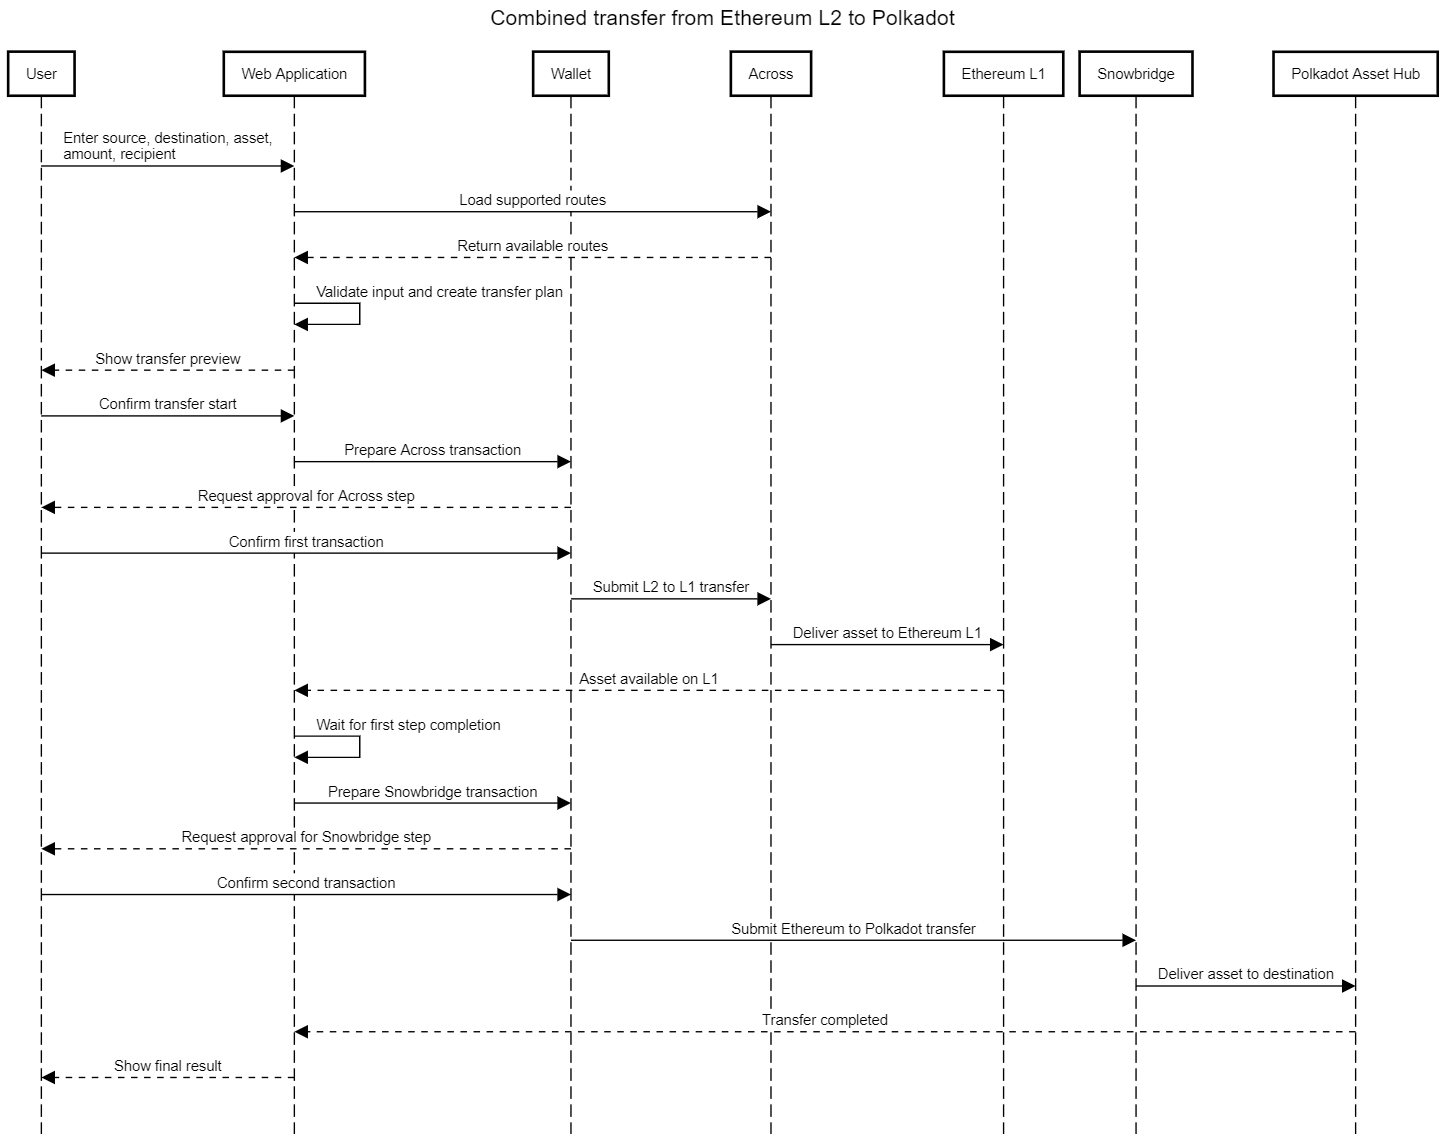
\includegraphics[width=\columnwidth]{L2 to Polkadot transfer.png}
    \caption{L2 to Polkadot transfer sequence diagram}
    \label{fig:l2-to-polkadot-transfer}
\end{figure}


\section{Evaluation and Discussion}


Since the proposed solution does not replace any interoperability protocols, the protocol properties such as bridge security, liquidity availability and transaction fees remain on the protocols themselfs.  The evaluation focuses on the application layer and on the on the practical behavior of the implemented workflow during testnet executions.

From workflow point of view, the proposed application firstly reduces the amount of interfaces the user has to work with in direct proportion with the number of protocols used which with scalability of the application can increase the workflow time in minutes. Also correct route is found instantly rather then pushing the user to research the correct way to transfer different tokens across different chains. 

\subsection{Testnet Execution Measurements}

To evaluate the practical behavior of the implementation, repeated transfers were performed in testnet environments. The tests were conducted on the same machine, an Asus Zenbook 14X, in a Google Chrome environment with the application running locally. 

The measured scenarios include transfers between Ethereum Layer 2 test networks, transfers from an Ethereum Layer 2 test network to Ethereum Layer 1, transfers from Ethereum Layer 1 to Westend Asset Hub and transfers from Ethereum L2 network to Westend Asset Hub. 

The metric was time measured after succesful transfers displayed by the application. This times were then taken and calculated into averages and ranges to have a clear overview of all measured transfer and ability to compare them.

User wallet confirmation were not considered to be part of the tested metric since the time to confirm could vary based on the response time of the user to confirmation in the included wallet.

%tabulku dat pod ten text nad tym
\begin{table}[H]
\centering
\caption{Observed execution times in testnet transfers}
\label{tab:testnet-execution-times}
\begin{tabular}{lccc}
\hline
Scenario & Avg. time & Range \\
\hline
L2 to L2 & 25.59 s & 24.95--27.07 s \\
L2 to L1 & 25.16 s & 24.38--25.75 s \\
L1 to Westend & 20 min 50 s & 20 min 14 s--21 min 26 s \\
L2 to Westend & 23 min 6 s & 22 min 6 s--24 min 32 s \\
\hline
\end{tabular}
\end{table}

As shown in in Table~\ref{tab:testnet-execution-times}. the transfer times across single Ethereum ecosystem were executed quickly and averaged around 25 seconds while transfers across different systems took significantly more and averaged around 22 minutes.

\subsection{Discussion}

The results from the testing shows a clear difference between token transfers performed inside the Ethereum ecosystem and transfers involving an external blockchain ecosystem. Transfers from L2 to L2 and L2 to L1(and vise versa) were executed and finished fast averaging around 25 seconds.
In contrast to this speeds the transfers from one ecosystem to another required significantly longer completion times exceeding 20 minutes on average. This results clearly show the higher latency in cross-ecosystem transfers than transfers executed within singe Ethereum environment.
The longest observed time was clearly transfers from L2 to Westend Asset Hub. However the transfer times were not much different from transfers only from L1 to Asset Hub since most of the time took transfer from L1 to Asset hub. But on the other hand it also shows that transfers are not longer when combined together and when executed separately.

These findings indicate that the proposed application does notprimarily improve protocol-level transfer speed but highly simplifies the coordination of multiple transfer steps into single simplier workflow. Simplification in workflow does indeed decrease transfer time when user inputs, having to find correct paths and applications are taken into consideration.

The presented measurements should not be taken as a unuversal performance benchmark, since they were measured in testnet environments and are highly dependent on network conditions, relayer behavior and also bridge availability.


\section{Conclusion}

This paper addressed the problem of fragmented asset transfers across Ethereum-based networks and the Polkadot ecosystem. Although existing interoperability protocols already provide mechanisms for cross-layer and cross-chain transfers, users are often required to manually combine multiple tools, interfaces, and transaction steps. This increases the complexity of the process and creates space for user errors.

The proposed solution introduced a client-side application layer that combines Across Protocol and Snowbridge into one guided transfer workflow. The implementation allows the user to define the source network, destination network, asset, amount, and recipient address, while the application prepares the required transfer plan and executes the necessary protocol steps in the correct order. In this way, the system does not replace the underlying interoperability protocols, but coordinates them through a unified user-facing process.

The evaluation showed that Ethereum-based transfers were completed significantly faster than transfers involving the Polkadot ecosystem. However, the main contribution of the proposed solution is not protocol-level performance improvement, but the simplification of multi-step transfer coordination. The application reduces the need for manual routing decisions and separates user input from protocol-specific execution details.

Future work may focus on extending the number of supported protocols, improving route selection based on fees and execution time. Additional monitoring of transaction states could also improve transparency during longer cross-ecosystem transfers. Since the proposed solution is scalable the application could be extended with more protocols and SDK to widen the transfer routes and connect even more chains with mindset to simplify the decision complexity and make overall experience easier for the end user.











%opisat aj vramci skalovatelnosti na dalsie sdk v pripade rozsirenia

%30 citacii
%ako by moje riesenie robi to 


%pozriet clanky novsie podobne riesenie, testy ako hnodnotit metriky

%\bibliographystyle{IEEEtran}
\bibliography{references}
\end{document}
